\documentclass[../DoAn.tex]{subfiles}
\begin{document}

Chương này đánh giá hệ thống trên hai giai đoạn: giai đoạn tĩnh đo hiệu
năng phân loại và phân tích sâu mô hình, giai đoạn động kiểm chứng khả
năng thu thập bằng chứng hành vi.

\section{Thiết lập thực nghiệm}
\label{section:5.1}

Quá trình đánh giá được tổ chức thành hai phần tương ứng hai giai đoạn
của hệ thống. Phần tĩnh sử dụng ba tập dữ liệu độc lập, thống kê trong
Bảng~\ref{tab:eval-datasets}.
\begin{table}[H]
\centering
\caption{Ba tập dữ liệu dùng trong đánh giá giai đoạn phân tích tĩnh.}
\label{tab:eval-datasets}
\begin{tabular}{|l|r|p{6cm}|}
\hline
\multicolumn{1}{|c|}{\textbf{Tập dữ liệu}} & \multicolumn{1}{c|}{\textbf{Số mẫu}} & \multicolumn{1}{c|}{\textbf{Mục đích}} \\
\hline
Holdout nội bộ & 40.328 &
  So sánh ba thuật toán trong cùng điều kiện (tách phân tầng 20\%
  tập huấn luyện, seed~42) \\
\hline
Mẫu kiểm thử riêng & 1.189 &
  Đánh giá theo bảy nhóm họ trên mẫu độc lập, không trùng tập huấn
  luyện (675 mã độc từ MalwareBazaar~\cite{malwarebazaar}, 514 lành tính) \\
\hline
EMBER 2024~\cite{joyce2025ember} & 119.992 &
  Đánh giá tổng quát hóa trên benchmark công khai, khác nguồn thu thập
  và ngoài phân phối (gần cân bằng) \\
\hline
\end{tabular}
\end{table}
Các độ đo gồm Accuracy, Precision, Recall, F1-Score, AUC-ROC và
AUC-PR. Do bài toán nhạy cảm với cả hai loại sai sót, hai chỉ số FPR
và FNR được theo dõi riêng.
Nhãn~1 (mã độc) được quy ước là lớp dương cần phát hiện, nhãn~0 là lành
tính.

Phần động được đánh giá trên 305~mẫu. Tập mã độc gồm 205~mẫu thu từ
MalwareBazaar~\cite{malwarebazaar}, phân bố trên bảy nhóm hành vi
(dropper, ransomware, trojan, RAT, worm, cryptominer, spyware) thuộc
36~họ; tập đối chứng gồm 100~ứng dụng mã nguồn mở hợp pháp. Mỗi mẫu được
thực thi trong cửa sổ quan sát 120~giây với cấu hình phần cứng tại
Mục~\ref{section:4.1}.

\section{Đánh giá giai đoạn phân tích tĩnh}
\label{section:5.2}

\subsection{So sánh ba thuật toán}
\label{section:5.2.1}

Ba thuật toán Random Forest, XGBoost và LightGBM được huấn luyện trên
toàn bộ 2.381 đặc trưng với cùng tập huấn luyện, sau đó đánh giá trên
tập holdout 40.328~mẫu (Bảng~\ref{tab:algo-comparison}).
\begin{table}[H]
\centering
\caption{So sánh ba thuật toán trên tập holdout 40.328~mẫu
  (toàn bộ 2.381 đặc trưng).}
\label{tab:algo-comparison}
\begin{tabular}{|l|c|c|c|c|c|c|}
\hline
\multicolumn{1}{|c|}{\textbf{Thuật toán}} & \multicolumn{1}{c|}{\textbf{Accuracy}} & \multicolumn{1}{c|}{\textbf{F1}} & \multicolumn{1}{c|}{\textbf{AUC-ROC}} & \multicolumn{1}{c|}{\textbf{FPR}} & \multicolumn{1}{c|}{\textbf{FNR}} \\
\hline
Random Forest & 0{,}9704 & 0{,}9709 & 0{,}9962 & 0{,}0429 & 0{,}0163 \\
\hline
XGBoost       & 0{,}9875 & 0{,}9875 & 0{,}9992 & \textbf{0{,}0144} & 0{,}0107 \\
\hline
\textbf{LightGBM} & \textbf{0{,}9876} & \textbf{0{,}9876} &
  \textbf{0{,}9993} & 0{,}0155 & \textbf{0{,}0094} \\
\hline
\end{tabular}
\end{table}
Hai mô hình boosting đạt kết quả cao hơn Random Forest trên mọi chỉ
số, với AUC-ROC lần lượt là 0{,}9993 và 0{,}9992 so với 0{,}9962.
Giữa hai mô hình boosting, LightGBM đạt F1 và AUC-ROC cao hơn, đồng
thời có FNR thấp nhất là 0{,}0094. Chỉ số FNR được ưu tiên vì bỏ sót
mã độc gây hậu quả nặng hơn báo động giả. Đường cong ROC
(Hình~\ref{fig:algo-roc}) cho thấy hai mô hình boosting sát nhau ở
vùng FPR thấp và nằm trên Random Forest. LightGBM được chọn cho các
bước tiếp theo.
\begin{figure}[H]
\centering
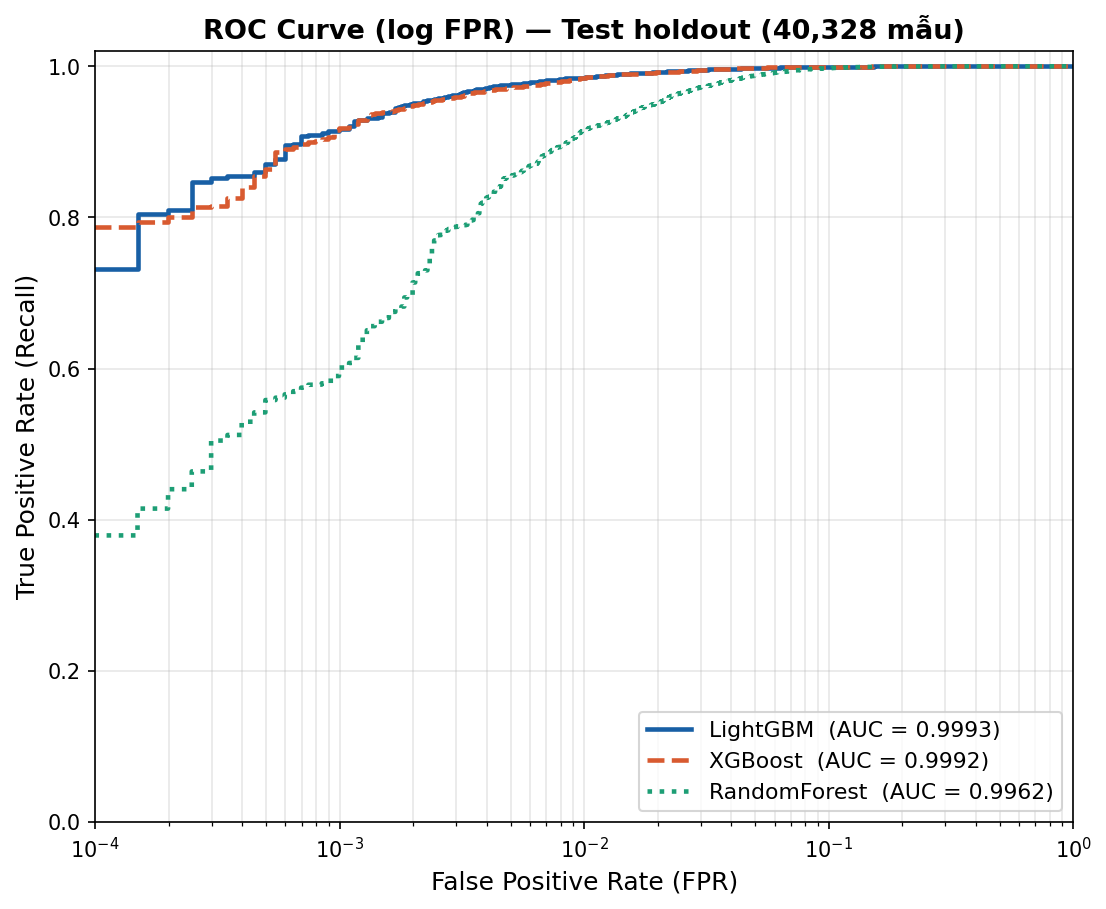
\includegraphics[width=0.9\textwidth]{Hinhve/Pic34AlgoROC.png}
\caption{Đường cong ROC của ba thuật toán trên tập holdout, trục FPR
  theo thang log.}
\label{fig:algo-roc}
\end{figure}
\subsection{Lựa chọn tập con đặc trưng}
\label{section:5.2.2}

Chỉ số Importance Gain của LightGBM được dùng để xếp hạng 2.381 đặc
trưng. Để định vị số chiều cần thiết, hiệu năng trên EMBER 2024 được
khảo sát nhanh qua mười lăm mốc từ 8 đến 2.381 đặc trưng, mỗi mốc huấn
luyện một lần (Hình~\ref{fig:feature-sweep}). Đường cong bão hòa từ
khoảng 64 đặc trưng: chỉ 96 chiều đã đạt trên 99{,}9\% F1 của mô hình
đầy đủ, sau đó khác biệt giữa các mốc nằm trong nhiễu thống kê
($\pm 0{,}003$). Cả ba ngưỡng 128, 256 và 384 đều nằm trên vùng bão hòa
này.
\begin{figure}[H]
\centering
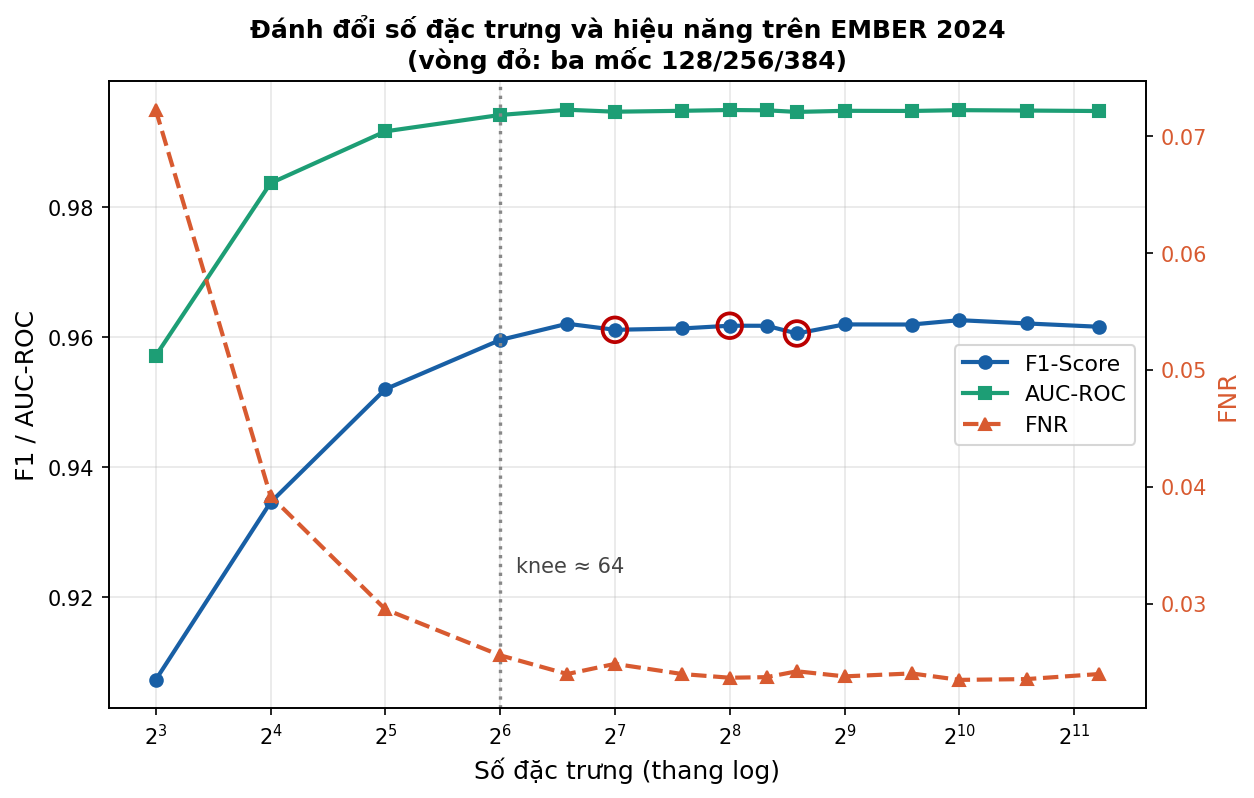
\includegraphics[width=0.9\textwidth]{Hinhve/Pic43FeatureSweep.png}
\caption{Đánh đổi số đặc trưng và hiệu năng trên EMBER 2024 qua mười lăm
  mốc; vòng đỏ đánh dấu ba ngưỡng 128/256/384, đường chấm dọc là điểm
  gãy (knee) tại 64 đặc trưng.}
\label{fig:feature-sweep}
\end{figure}
Ba ngưỡng được huấn luyện lại đầy đủ bằng 5-fold cross-validation và so
sánh với mô hình 2.381 chiều (Bảng~\ref{tab:feature-selection},
119.992~mẫu EMBER 2024).
\begin{table}[H]
\centering
\caption{So sánh bốn cấu hình đặc trưng trên tập EMBER 2024
  (119.992~mẫu).}
\label{tab:feature-selection}
\begin{tabular}{|l|c|c|c|c|c|}
\hline
\multicolumn{1}{|c|}{\textbf{Cấu hình}} & \multicolumn{1}{c|}{\textbf{Số chiều}} & \multicolumn{1}{c|}{\textbf{Accuracy}} & \multicolumn{1}{c|}{\textbf{F1}} & \multicolumn{1}{c|}{\textbf{AUC-ROC}} & \multicolumn{1}{c|}{\textbf{FNR}} \\
\hline
Full          & 2.381 & 0{,}9613 & 0{,}9618 & 0{,}9948 & 0{,}0241 \\
\hline
Top-128       & 128   & 0{,}9608 & 0{,}9614 & 0{,}9947 & 0{,}0247 \\
\hline
Top-256       & 256   & 0{,}9603 & 0{,}9609 & 0{,}9946 & 0{,}0249 \\
\hline
\textbf{Top-384} & 384 & 0{,}9610 & 0{,}9615 & 0{,}9948 & 0{,}0241 \\
\hline
\end{tabular}
\end{table}
Bốn cấu hình cho hiệu năng tương đương: chênh lệch F1 giữa Top-384 và
Full chỉ 0{,}0003, AUC-ROC bằng nhau ở 0{,}9948 dù số chiều giảm hơn
sáu lần. So với holdout nội bộ, F1 giảm từ 0{,}9876 xuống 0{,}9615,
phản ánh độ khó khi tổng quát hóa sang dữ liệu khác nguồn, ngoài phân phối.
Việc giảm chiều không làm mô hình nhẹ hay nhanh hơn, vì kích thước và
độ trễ phụ thuộc số cây chứ không phải số chiều; lợi ích là tập đặc
trưng gọn và dễ diễn giải hơn. Trong ba cấu hình rút gọn, Top-384 đạt
F1 và AUC-ROC cao nhất, đồng thời FNR thấp nhất 0{,}0241 bằng đúng mô
hình đầy đủ; do bỏ sót mã độc là sai sót cần ưu tiên giảm, Top-384 được
chọn triển khai.

Tỉ lệ phát hiện theo nhóm của mô hình Top-384 trên tập kiểm thử riêng
được trình bày trong Bảng~\ref{tab:family-detection} và
Hình~\ref{fig:family-detection}.
\begin{table}[H]
\centering
\caption{Tỉ lệ phát hiện theo nhóm của mô hình Top-384
  (tập kiểm thử riêng).}
\label{tab:family-detection}
\begin{tabular}{|l|c|l|c|}
\hline
\multicolumn{1}{|c|}{\textbf{Nhóm}} & \multicolumn{1}{c|}{\textbf{Tỉ lệ}} & \multicolumn{1}{c|}{\textbf{Nhóm}} & \multicolumn{1}{c|}{\textbf{Tỉ lệ}} \\
\hline
Lành tính (benign) & 99{,}6\% & RAT        & 92{,}8\% \\
\hline
Ransomware         & 98{,}9\% & Trojan     & 89{,}6\% \\
\hline
Worm               & 97{,}0\% & Cryptominer & 87{,}6\% \\
\hline
Spyware            & 99{,}0\% & Dropper    & 91{,}2\% \\
\hline
\end{tabular}
\end{table}
Mô hình đạt tỉ lệ phát hiện quanh 99\% trên nhóm lành tính, ransomware
và spyware, nhưng thấp hơn ở cryptominer (87{,}6\%) và trojan
(89{,}6\%). Hai nhóm này thường tái sử dụng cấu trúc PE gần với phần
mềm hợp pháp, làm giảm khả năng phân biệt của đặc trưng tĩnh và là lý
do cần bổ sung giai đoạn phân tích động.
\begin{figure}[H]
\centering
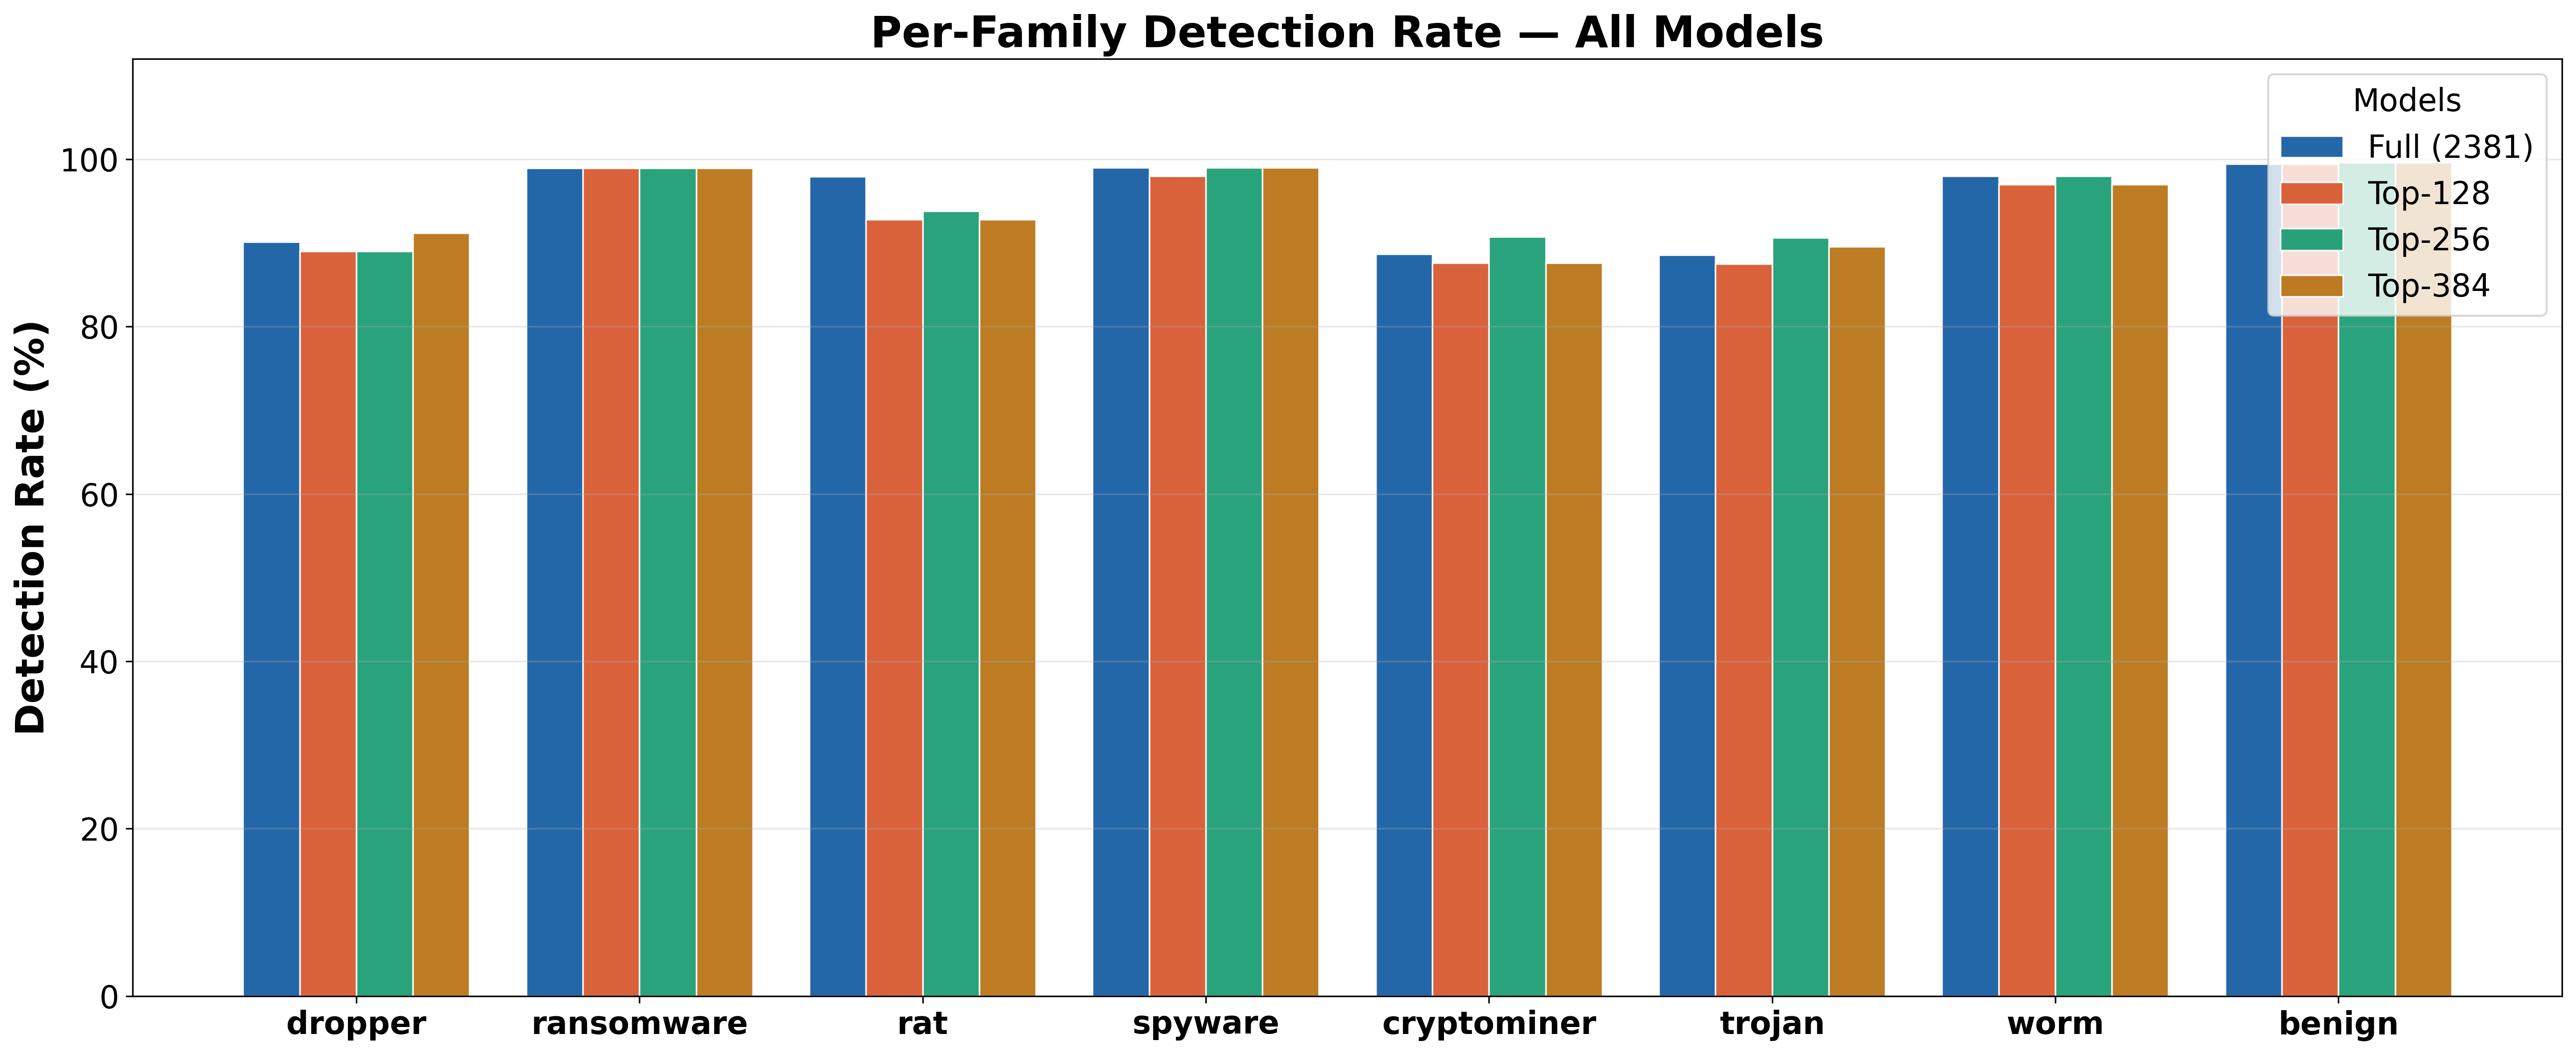
\includegraphics[width=1.0\textwidth]{Hinhve/Pic39Family.png}
\caption{Tỉ lệ phát hiện theo nhóm của bốn cấu hình đặc trưng.}
\label{fig:family-detection}
\end{figure}
Kết quả này phù hợp với các công trình trên dòng đặc trưng EMBER. Anderson
và Roth đạt AUC-ROC 0{,}9991 trên EMBER-2018~\cite{ember2018}; Choudhary và
cộng sự đạt 97{,}52\% độ chính xác khi rút gọn còn 384 chiều~\cite{choudhary2025}
--- cả hai đánh giá trên dữ liệu cùng thời kỳ huấn luyện. Mô hình Top-384 của
đồ án đạt AUC-ROC 0{,}9948 và 96{,}10\% độ chính xác trên EMBER 2024, bộ dữ
liệu mới hơn và khó hơn do nằm ngoài phân phối. Mức chênh nhỏ trên tập khó
hơn cho thấy mô hình tổng quát hóa tốt.

\subsection{Tối ưu ngưỡng phân loại}
\label{section:5.2.3}

Ba mục dưới đây phân tích sâu mô hình Top-384 đã chọn triển khai, nhằm
phản ánh đúng hành vi của mô hình vận hành.

Ngưỡng quyết định $\tau$ điều tiết đánh đổi giữa FPR và FNR. Xác suất
dự đoán được quét trên 99~ngưỡng cách đều từ 0{,}01 đến 0{,}99, tại mỗi
ngưỡng tính FPR, FNR và F1. Từ đường quét này chọn ba mốc tiêu biểu để
so sánh: ngưỡng mặc định 0{,}50 theo quy ước thông dụng; ngưỡng tối ưu
F1 là điểm cho F1 cao nhất (0{,}88); và ngưỡng ưu tiên an toàn là điểm
có FPR thấp nhất trong số các ngưỡng
giữ FNR~$\leq 2\%$ (0{,}33). Bảng~\ref{tab:threshold} và
Hình~\ref{fig:threshold} so sánh ba mốc này trên tập EMBER 2024.
\begin{table}[H]
\centering
\caption{So sánh ba mốc ngưỡng phân loại trên tập EMBER 2024.}
\label{tab:threshold}
\begin{tabular}{|l|c|c|c|c|c|}
\hline
\multicolumn{1}{|c|}{\textbf{Ngưỡng}} & \multicolumn{1}{c|}{\textbf{$\tau$}} & \multicolumn{1}{c|}{\textbf{Accuracy}} & \multicolumn{1}{c|}{\textbf{F1}} & \multicolumn{1}{c|}{\textbf{FPR}} & \multicolumn{1}{c|}{\textbf{FNR}} \\
\hline
Mặc định          & 0{,}50 & 0{,}9610 & 0{,}9615 & 0{,}0540 & 0{,}0241 \\
\hline
Tối ưu F1         & 0{,}88 & 0{,}9660 & 0{,}9658 & 0{,}0276 & 0{,}0404 \\
\hline
Ưu tiên an toàn   & 0{,}33 & 0{,}9573 & 0{,}9582 & 0{,}0655 & 0{,}0199 \\
\hline
\end{tabular}
\end{table}
Ngưỡng 0{,}88 cho F1 cao nhất nhưng FNR tăng lên 0{,}0404, tức bỏ sót
nhiều mã độc hơn. Ngưỡng 0{,}33 đưa FNR xuống mức thấp nhất là
0{,}0199, đổi lại FPR tăng lên 0{,}0655. Hệ thống chọn $\tau = 0{,}33$
theo định hướng ưu tiên an toàn, do bỏ sót mã độc gây hậu quả nặng hơn
báo động giả. Phần báo động giả tăng thêm được giai đoạn động sàng lọc
qua nhãn \texttt{suspicious} (Mục~\ref{section:5.3.3}).
\begin{figure}[H]
\centering
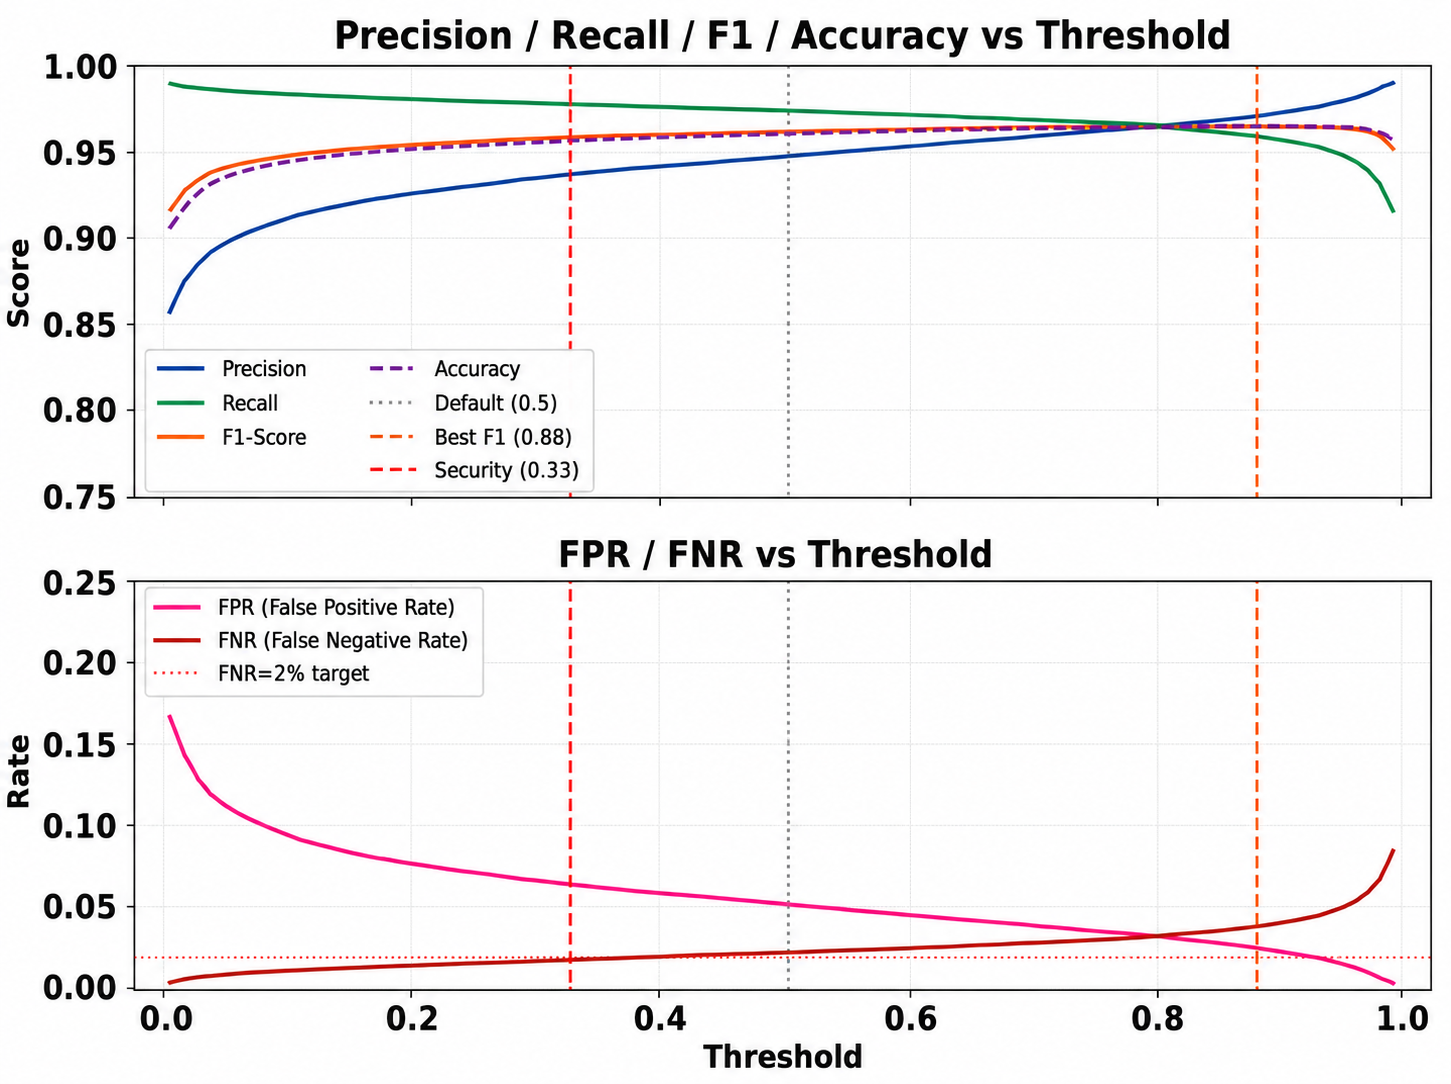
\includegraphics[width=1.0\textwidth]{Hinhve/Pic36Threshold.png}
\caption{Biến thiên FPR và FNR theo ngưỡng phân loại.}
\label{fig:threshold}
\end{figure}
\subsection{Phân tích đặc trưng}
\label{section:5.2.4}

Giá trị SHAP được tính trên mẫu con ngẫu nhiên 2.000 phần tử (seed~42)
rồi tổng hợp theo chín nhóm đặc trưng EMBER, nhằm xác định nhóm ảnh
hưởng nhiều nhất đến quyết định của mô hình Top-384
(Hình~\ref{fig:shap-group}). Do \texttt{TreeExplainer} có chi phí lớn
trên từng mẫu, việc lấy mẫu con là cần thiết; với mục tiêu đo mức đóng
góp tổng thể (trung bình trị tuyệt đối SHAP theo nhóm), 2.000 mẫu đã đủ
cho ước lượng ổn định mà không phải chạy trên toàn tập.
\begin{figure}[H]
\centering
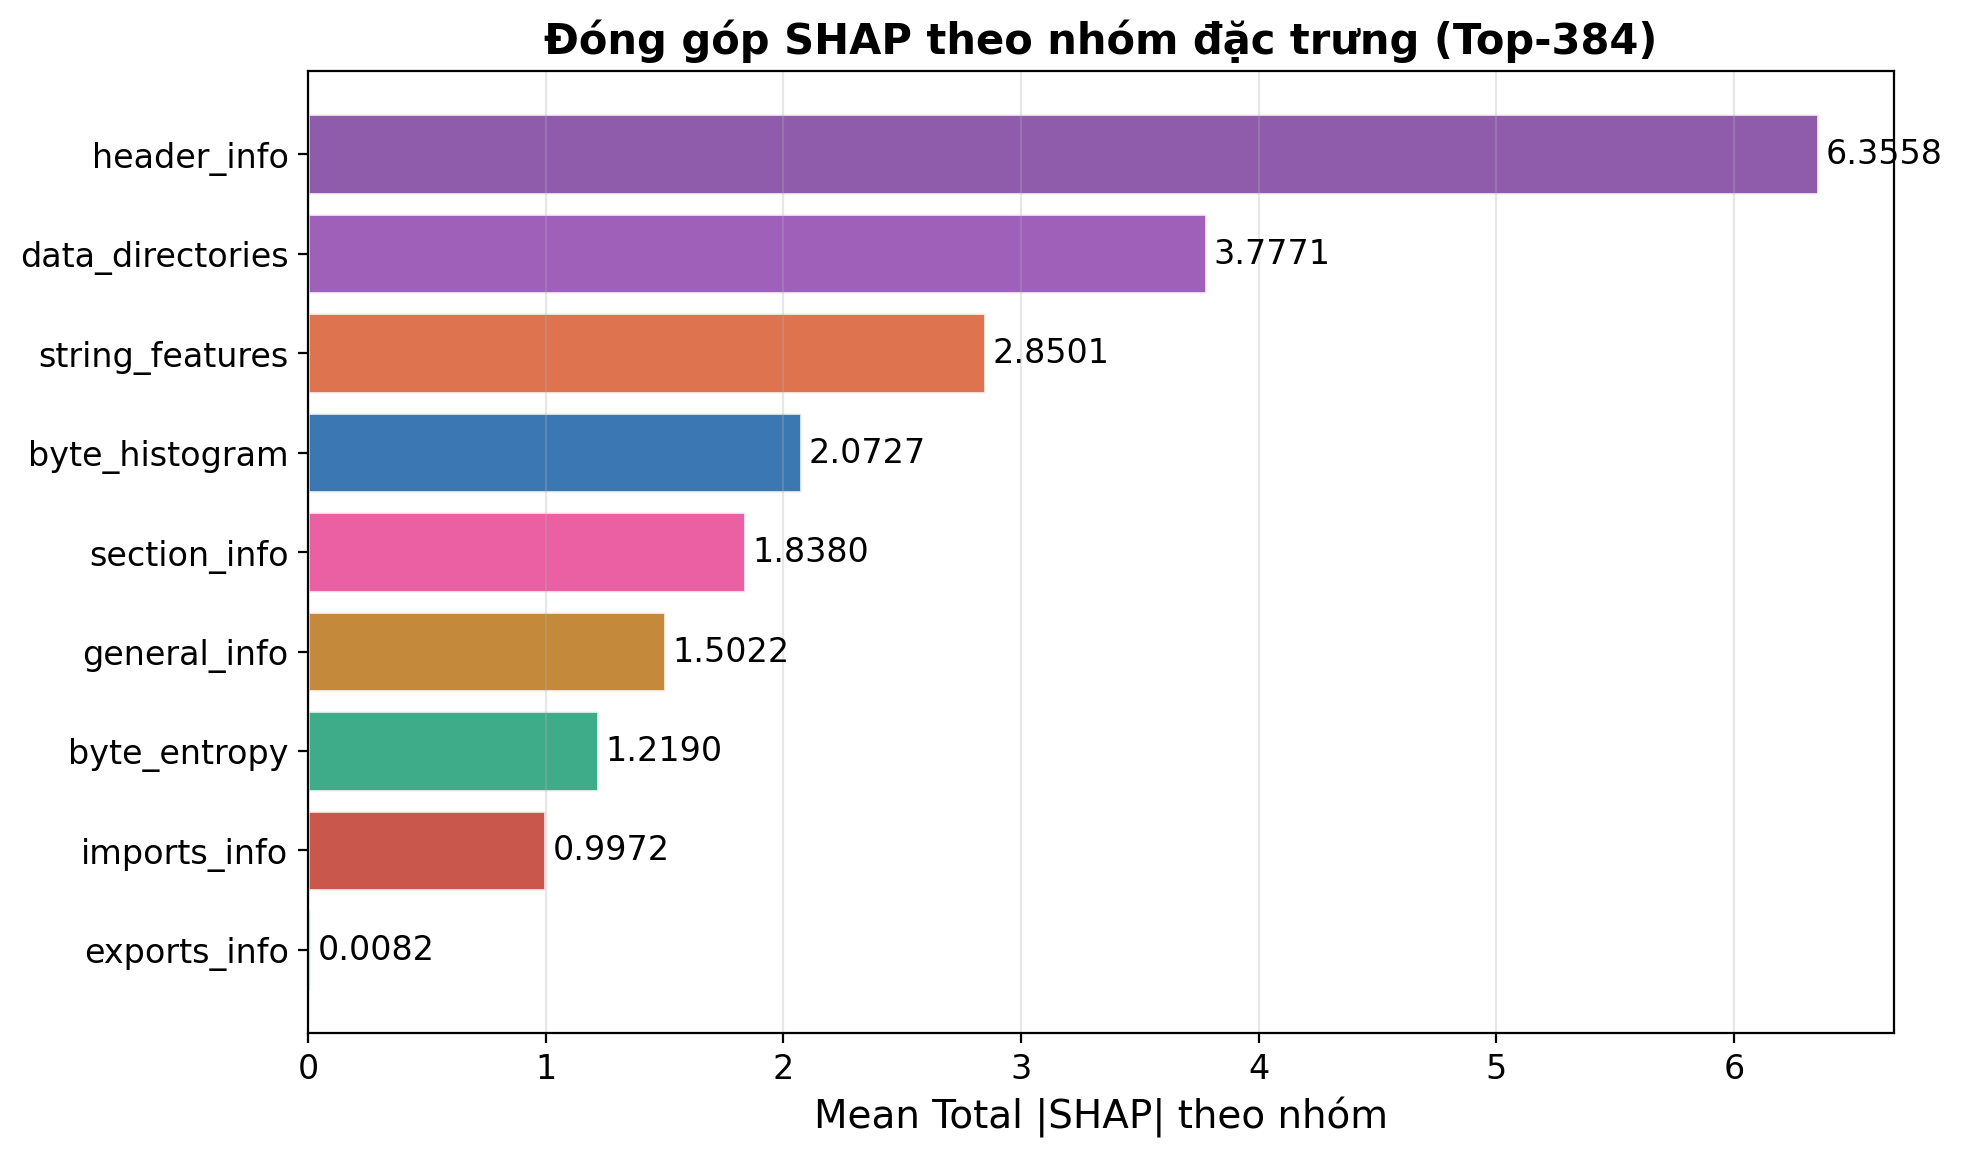
\includegraphics[width=1.0\textwidth]{Hinhve/Pic37ShapGroup.png}
\caption{Tổng giá trị SHAP tuyệt đối theo nhóm đặc trưng.}
\label{fig:shap-group}
\end{figure}
Hai nhóm \textit{header\_info} và \textit{data\_directories} đóng góp
lớn nhất, với tổng giá trị SHAP lần lượt là 6{,}36 và 3{,}78. Kết quả
cho thấy mô hình dựa chủ yếu vào các trường cấu trúc trong PE header và
bảng data directories, vốn phản ánh cách tệp được liên kết và đóng gói.
Các nhóm \textit{string\_features}, \textit{byte\_histogram} và
\textit{section\_info} đóng vai trò bổ trợ, còn \textit{exports\_info}
gần như không đóng góp do phần lớn tệp không có bảng export. Việc đóng
góp tập trung ở một số nhóm giải thích vì sao tập rút gọn 384 chiều
duy trì được hiệu năng.

\subsection{Phân tích lỗi}
\label{section:5.2.5}

Phân tích lỗi được thực hiện tại ngưỡng mặc định 0{,}5, dùng làm mốc
trung lập để khảo sát cấu trúc lỗi (không phải ngưỡng triển khai 0{,}33).
Tại mốc này, trên tập EMBER 2024 mô hình Top-384 sinh 1.444 trường hợp
bỏ sót (FN) và 3.240 báo động giả (FP); các mức 0{,}1, 0{,}3 hay 0{,}9
nêu dưới đây là khoảng điểm dự đoán, không phải ngưỡng phân loại. Phân
bố hai loại lỗi theo khoảng điểm được trình bày trong
Hình~\ref{fig:error-dist}.
Trong nhóm bỏ sót, 54\% có điểm dưới 0{,}1, tức mô hình gán điểm rất
thấp cho mẫu mã độc. Các mẫu này có cấu trúc PE gần với phần mềm lành
tính, đặc trưng của kỹ thuật đóng gói và làm rối mã đã nêu tại
Mục~\ref{section:2.2.2}, nên không thể khắc phục bằng điều chỉnh ngưỡng.
Phần 46\% còn lại có điểm cao hơn, gần ngưỡng 0{,}5; trong đó các mẫu
thuộc khoảng $[0{,}3; 0{,}5)$ được thu hồi khi hạ ngưỡng về 0{,}33, giúp
phát hiện thêm 249 mã độc so với ngưỡng 0{,}5 --- đây chính là cơ sở
định lượng cho lựa chọn $\tau = 0{,}33$ ở Mục~\ref{section:5.2.3}. Trong
nhóm báo động giả, 47\% có điểm trên 0{,}9 và rơi vào phần mềm hợp pháp
có cấu trúc gần với mã độc, phần còn lại có điểm gần ngưỡng 0{,}5. Cả hai loại lỗi đều xuất phát từ giới
hạn của phân tích tĩnh và là cơ sở cho vai trò bổ sung của giai đoạn
động.
\begin{figure}[H]
\centering
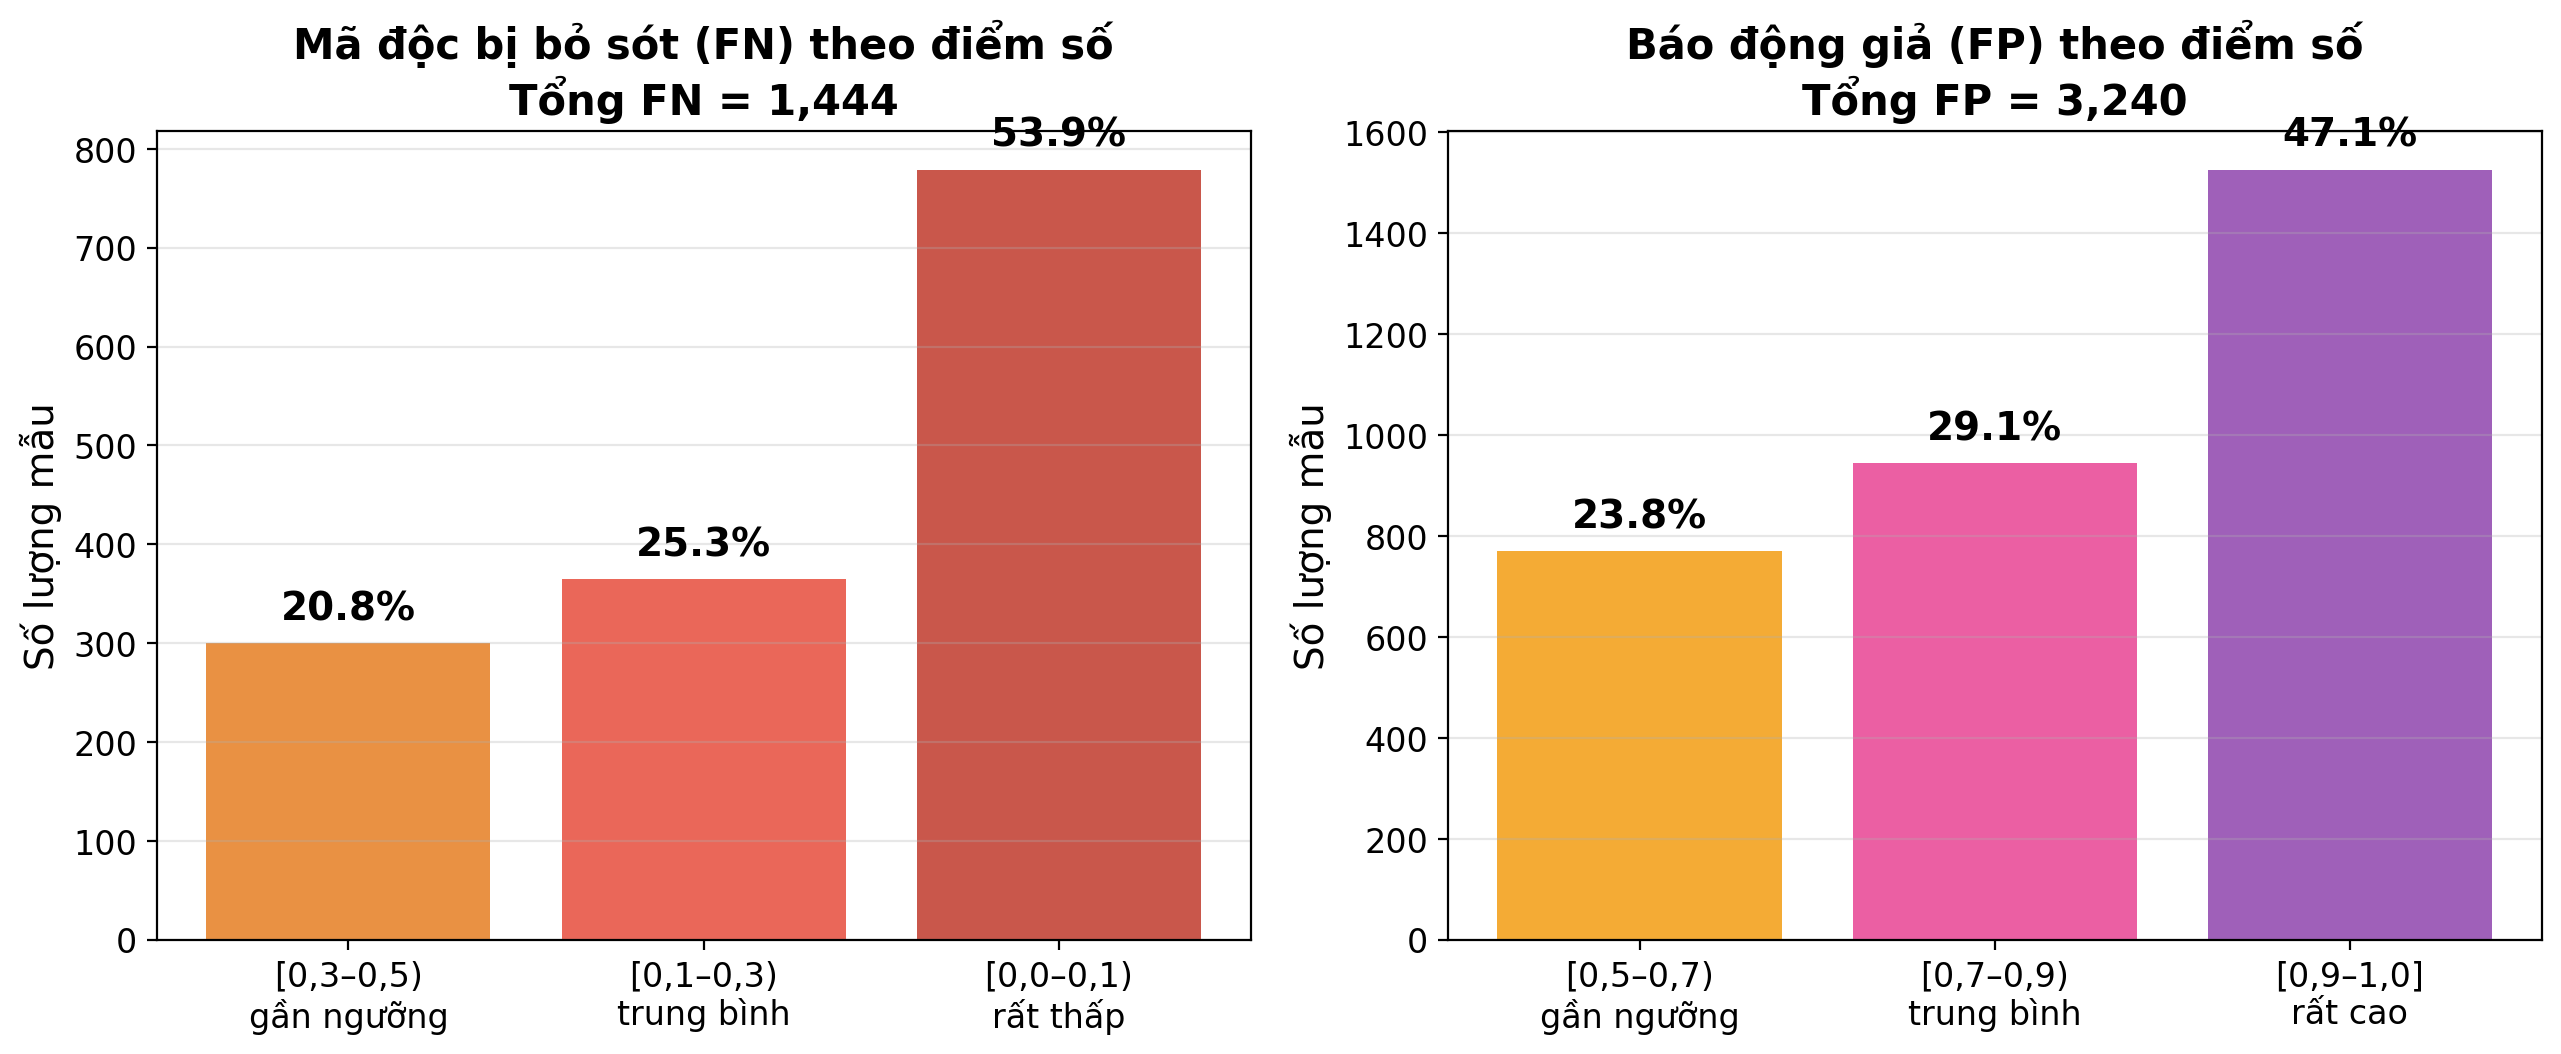
\includegraphics[width=1.0\textwidth]{Hinhve/Pic40ErrorDist.png}
\caption{Phân bố các trường hợp phân loại sai theo khoảng điểm số
  (FN bên trái, FP bên phải).}
\label{fig:error-dist}
\end{figure}

\subsection{Hiệu chuẩn độ tin cậy}
\label{section:5.2.6}

Độ chính xác phân loại chỉ phản ánh nhãn dự đoán đúng hay sai, không bảo đảm
con số xác suất xuất ra phản ánh đúng tần suất thực tế. Để con số độ tin cậy
hiển thị có ý nghĩa, xác suất thô của mô hình Top-384 được đối chiếu với tỉ lệ
mã độc thực tế theo từng khoảng điểm trên tập EMBER 2024
(Bảng~\ref{tab:calibration-bins}). Trong mỗi khoảng điểm, cột ``điểm trung
bình'' là xác suất trung bình mà mô hình gán cho các mẫu thuộc khoảng đó,
còn cột ``tỉ lệ mã độc thực tế'' là phần mẫu thực sự là mã độc theo nhãn.
Mô hình được hiệu chuẩn tốt khi hai con số này xấp xỉ nhau; chênh lệch lớn
nghĩa là xác suất xuất ra chưa phản ánh đúng rủi ro thật.
\begin{table}[H]
\centering
\caption{Đối chiếu điểm dự đoán với tỉ lệ thực tế (trích các khoảng tiêu biểu,
  thống kê trên nửa tập kiểm EMBER 2024 dùng đánh giá hiệu chuẩn,
  khoảng 60.000~mẫu). Vùng điểm cực thấp và cực cao khớp tốt, vùng giữa tự
  tin thái quá.}
\label{tab:calibration-bins}
\begin{tabular}{|c|r|c|c|}
\hline
\multicolumn{1}{|c|}{\textbf{Khoảng điểm}} & \multicolumn{1}{c|}{\textbf{Số mẫu}} & \multicolumn{1}{c|}{\textbf{Điểm trung bình}} & \multicolumn{1}{c|}{\textbf{Tỉ lệ mã độc thực tế}} \\
\hline
0{,}0--0{,}1 & 27.474 & 0{,}004 & 0{,}013 \\
\hline
0{,}3--0{,}4 & 322    & 0{,}350 & 0{,}270 \\
\hline
0{,}7--0{,}8 & 340    & 0{,}751 & 0{,}397 \\
\hline
0{,}8--0{,}9 & 505    & 0{,}854 & 0{,}455 \\
\hline
0{,}9--1{,}0 & 29.515 & 0{,}997 & 0{,}975 \\
\hline
\end{tabular}
\end{table}
Khoảng 95\% mẫu trong nửa tập kiểm rơi vào hai vùng cực (điểm dưới 0{,}1
hoặc trên 0{,}9), nơi con số khớp tốt với thực tế. Tuy nhiên ở vùng lưỡng lự, mô hình tự tin thái
quá rõ rệt: nhóm điểm 0{,}8--0{,}9 có điểm trung bình 0{,}854 nhưng thực tế chỉ
45{,}5\% là mã độc. Xác suất được hiệu chuẩn bằng Isotonic Regression (học trên
một nửa tập, kiểm trên nửa còn lại); sai số hiệu chuẩn kỳ vọng (ECE) giảm từ
0{,}0249 xuống 0{,}0022 (Hình~\ref{fig:calibration}). Do phép hiệu chuẩn đơn
điệu, thứ tự xếp hạng các mẫu không đổi nên nhãn phân loại và các độ đo ở những
mục trước được giữ nguyên; chỉ con số độ tin cậy hiển thị trở nên đáng tin.
\begin{figure}[H]
\centering
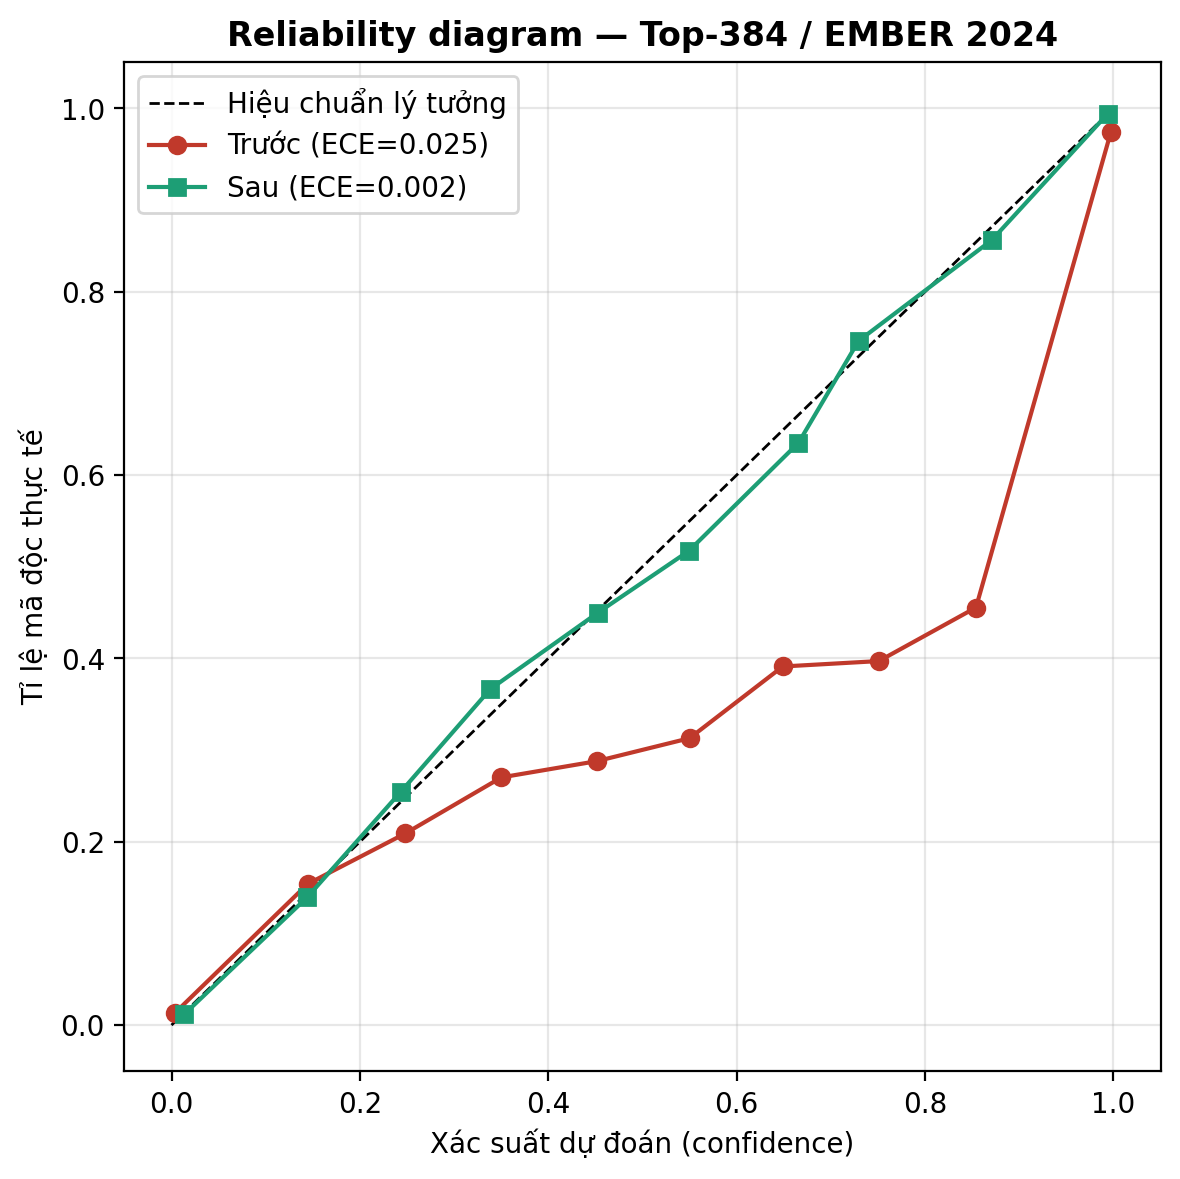
\includegraphics[width=0.7\textwidth]{Hinhve/Pic45Calibration.png}
\caption{Reliability diagram của mô hình Top-384 trước và sau hiệu chuẩn trên
  tập EMBER 2024.}
\label{fig:calibration}
\end{figure}
\section{Đánh giá giai đoạn phân tích động}
\label{section:5.3}

Mục tiêu đánh giá ở giai đoạn động khác với giai đoạn tĩnh: thay vì đo
lại độ chính xác phân loại, phần này kiểm chứng khả năng thu thập bằng
chứng hành vi của mẫu khi thực thi. Tập đánh giá gồm 205~mẫu mã độc trải trên
bảy nhóm hành vi (36~họ) và 100~ứng dụng hợp pháp. Hai tập đóng vai trò
khác nhau: 205~mẫu mã độc dùng đo độ phủ bằng chứng và khả năng phát
hiện hành vi (Mục~\ref{section:5.3.1}, \ref{section:5.3.4}), còn
100~ứng dụng hợp pháp dùng đo tỉ lệ dương tính giả
(Mục~\ref{section:5.3.3}, \ref{section:5.3.4}). Cả 305~phiên đều hoàn
tất và sinh báo cáo, mỗi phiên ghi nhận trung bình 162~sự kiện chuẩn hóa
từ Sysmon và SilkETW, gồm sự kiện tiến trình, tệp, registry, mạng và nạp
assembly.

\subsection{Độ phủ bằng chứng hành vi}
\label{section:5.3.1}

Theo lượng bằng chứng thu được, các mẫu mã độc được chia thành ba mức
theo tín hiệu quan sát được (Hình~\ref{fig:dyn-tiers}). Mức rõ ràng
(147~mẫu, chiếm 72\%) gồm các mẫu bộc lộ ít nhất một tín hiệu có ý
nghĩa: kỹ thuật ATT\&CK, kết nối mạng, thao tác registry, tạo từ ba tệp
trở lên, hoặc xóa tệp. Mức trung bình (24~mẫu) không đạt mức trên nhưng
vẫn sinh tiến trình con hoặc tạo một--hai tệp. Mức không bộc lộ (34~mẫu)
không để lại tín hiệu nào, chủ yếu thuộc các họ có cơ chế né sandbox,
phù hợp với phạm vi giới hạn tại Chương~\ref{chapter:Introduction}.

Xét độ phủ trên bảy loại hành vi quan sát được --- tạo tệp, tiêm mã,
cây tiến trình, xóa tệp, sửa registry, kết nối mạng và duy trì hiện diện
(Hình~\ref{fig:dyn-coverage}) --- thì tạo tệp, tiêm mã và cây tiến trình
phổ biến nhất, lần lượt xuất hiện ở 134, 107 và 105~mẫu. Kết nối mạng và
duy trì hiện diện ít gặp hơn do phụ thuộc vào máy chủ điều khiển hoặc
điều kiện kích hoạt.
\begin{figure}[H]
\centering
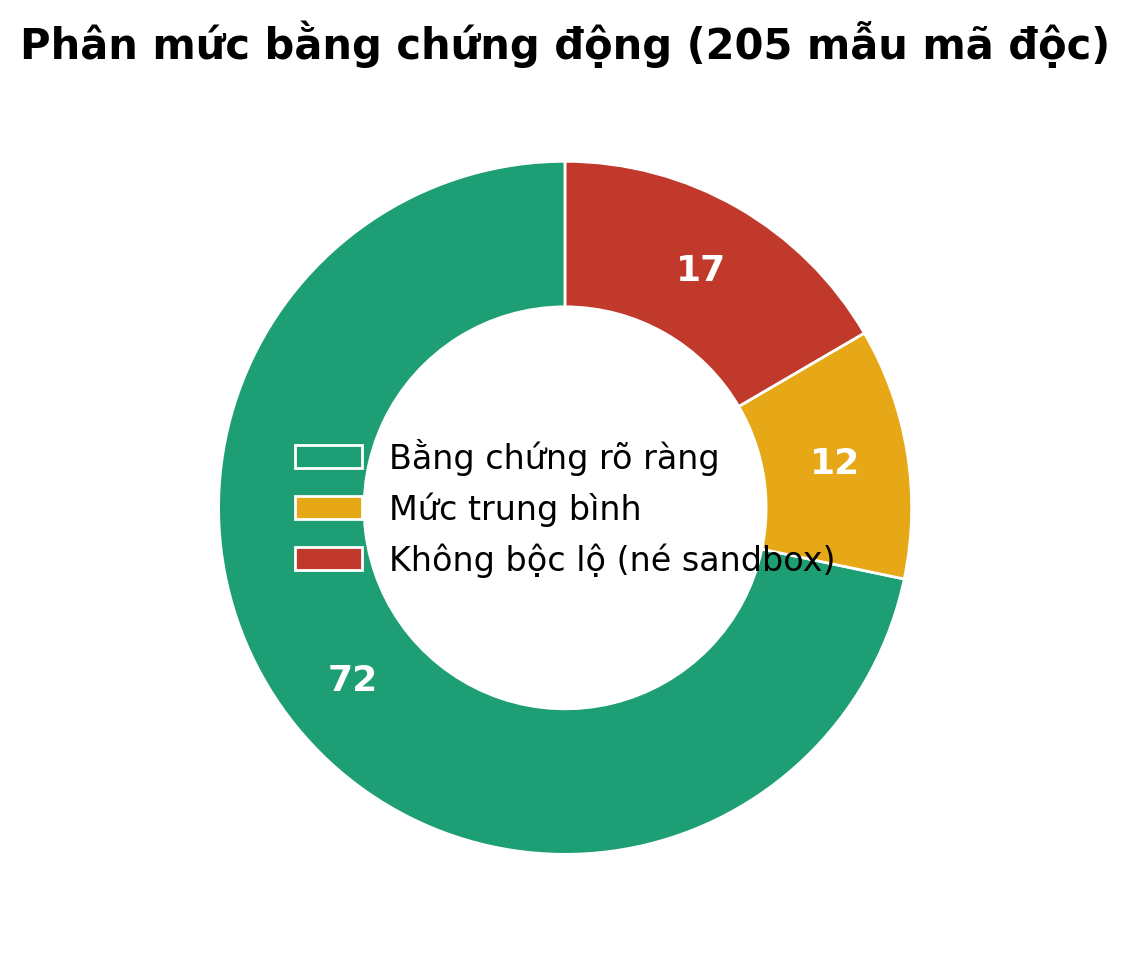
\includegraphics[width=0.6\textwidth]{Hinhve/Pic42DynTiers.png}
\caption{Phân mức bằng chứng động trên 205~mẫu mã độc.}
\label{fig:dyn-tiers}
\end{figure}
\begin{figure}[H]
\centering
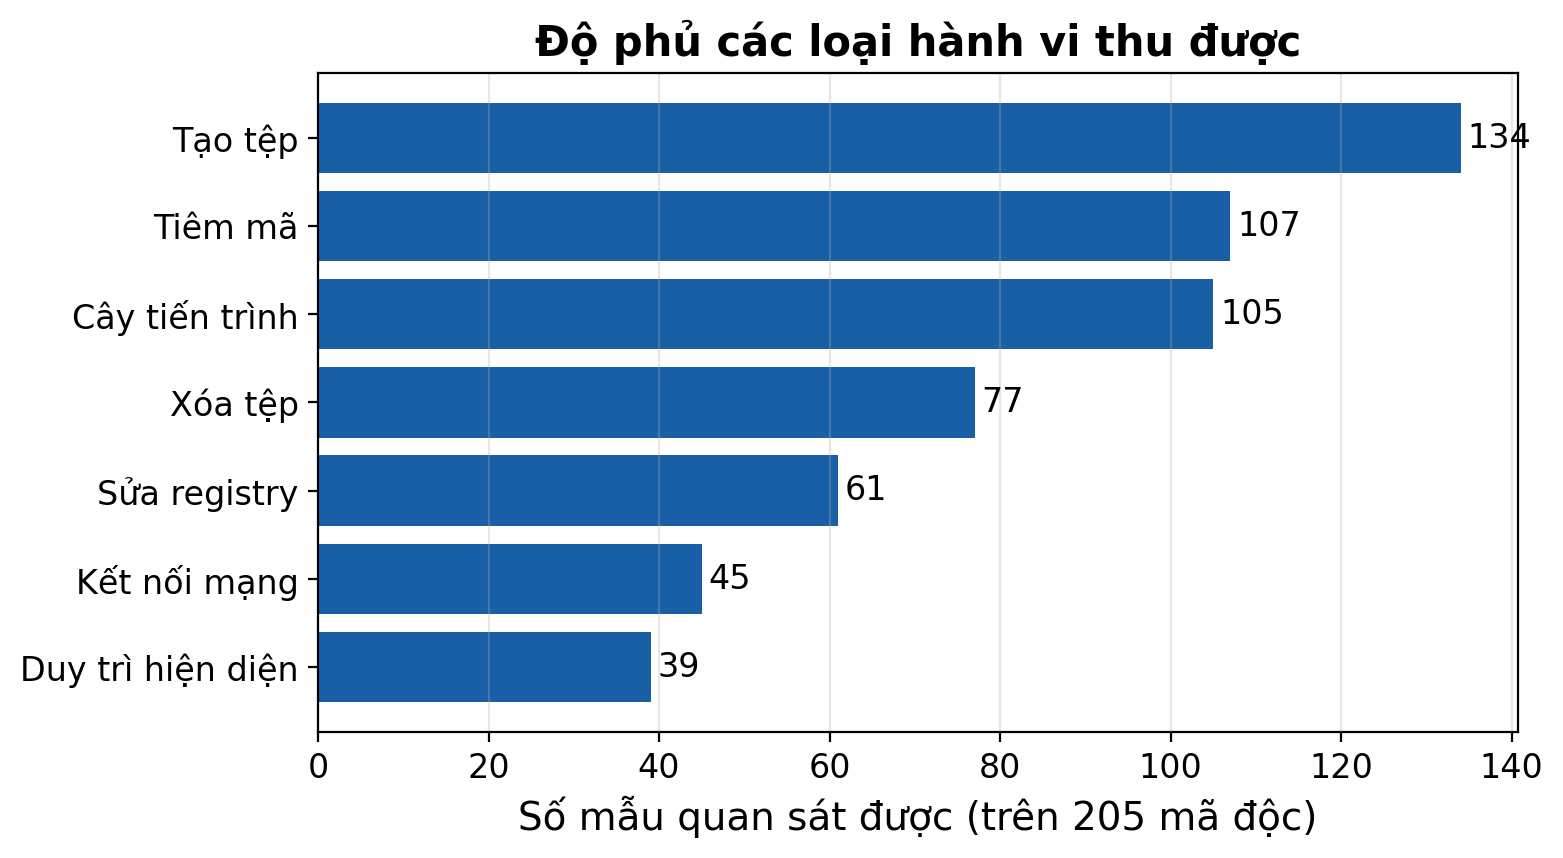
\includegraphics[width=1.0\textwidth]{Hinhve/Pic41DynCoverage.png}
\caption{Độ phủ các loại hành vi thu được.}
\label{fig:dyn-coverage}
\end{figure}
\subsection{Bằng chứng hành vi qua các mẫu đại diện}
\label{section:5.3.2}

Bằng chứng động của một số mẫu mã độc tiêu biểu được trình bày trong
Bảng~\ref{tab:dyn-cases}. Mỗi dòng liệt kê chỉ số xâm phạm và kỹ thuật
ATT\&CK trích xuất trực tiếp từ phiên thực thi.
\begin{table}[H]
\centering
\caption{Bằng chứng hành vi của các mẫu mã độc đại diện.}
\label{tab:dyn-cases}
\begin{tabular}{|l|>{\raggedright\arraybackslash}p{7cm}|>{\raggedright\arraybackslash}p{3cm}|}
\hline
\multicolumn{1}{|c|}{\textbf{Mẫu}} & \multicolumn{1}{c|}{\textbf{Bằng chứng động}} & \multicolumn{1}{c|}{\textbf{ATT\&CK}} \\
\hline
Phobos (ransomware) &
  Mã hóa tệp đuôi \texttt{.id[\ldots].[email].eight}; xóa hàng loạt
  tệp và bản sao lưu; ghi khóa Run; tiêm mã 9 tiến trình &
  T1055, T1070, T1218, T1547.001 \\
\hline
STOP (ransomware) &
  Kết nối C2 \texttt{api.2ip.ua}, \texttt{asvb.top}; giả mạo tiến
  trình (process hollowing); tự sao chép vào \texttt{AppData}; ghi
  khóa Run \texttt{SysHelper} &
  T1003.001, T1055, T1055.012, T1547.001 \\
\hline
Babuk (ransomware) &
  Tắt tường lửa (\texttt{netsh advfirewall}); ghi tệp
  \texttt{ransom\_message.txt}; tiêm mã 11 tiến trình &
  T1055, T1218, T1547.001 \\
\hline
Sality (virus lây nhiễm) &
  Vô hiệu hóa tường lửa; tiêm mã vào khoảng 140 tiến trình; cài dịch
  vụ tự khởi động; truy cập LSASS &
  T1003.001, T1055, T1543.003 \\
\hline
NetWire (RAT) &
  Lạm dụng \texttt{RegSvcs.exe} (.NET) để thực thi; thả tệp
  \texttt{.exe} và \texttt{.vbs}; ghi khóa Run &
  T1055, T1218, T1547.001 \\
\hline
\end{tabular}
\end{table}
Các bằng chứng này tái hiện đúng đặc trưng của từng họ: ransomware
(Phobos, STOP, Babuk) mã hóa tệp, xóa bản sao lưu hoặc tắt phòng thủ
và cố thủ qua khóa Run; virus lây nhiễm (Sality) tiêm mã diện rộng vào
hàng trăm tiến trình và cài dịch vụ tự khởi động; RAT (NetWire) lạm
dụng tệp hệ thống .NET để thực thi rồi duy trì hiện diện. Kết quả cho
thấy giai đoạn động tái hiện hành vi của mẫu ở mức có thể diễn giải và
truy vết.

\subsection{Đánh giá pipeline tích hợp}
\label{section:5.3.3}

Kết luận cuối được tổng hợp từ cả hai giai đoạn. Trên 205~mẫu mã độc,
hệ thống xác định đúng 204~mẫu (200 nhãn \texttt{malware}, 4 nhãn
\texttt{suspicious}); mẫu bỏ sót duy nhất là một mẫu Babuk có xác suất
tĩnh sát ngưỡng và không bộc lộ hành vi. Trên 100~ứng dụng hợp pháp,
83~mẫu được kết luận lành tính, 9~mẫu bị gắn nhãn \texttt{suspicious} và
8~mẫu bị quy thành \texttt{malware}. Phần lớn mẫu \texttt{malware} là các
tiện ích mã hóa và gỡ lỗi bị giai đoạn tĩnh chấm điểm cao do cấu trúc gần
với mã độc; các nhãn \texttt{suspicious} đến từ phần mềm hợp pháp có thao
tác truy cập tiến trình. Tỉ lệ dương tính giả theo kỹ thuật được trình bày
tại Mục~\ref{section:5.3.4}.

Một số mẫu thuộc các họ có cơ chế né tránh không bộc lộ hành vi trong
sandbox nhưng vẫn được kết luận mã độc nhờ giai đoạn tĩnh, kèm cảnh báo
nghi ngờ né tránh. Trường hợp này thể hiện vai trò bổ sung giữa hai
giai đoạn: khi một giai đoạn không thu được tín hiệu, giai đoạn còn lại
vẫn giữ được kết luận.

Quy mô đánh giá động là 305~mẫu, giới hạn bởi chi phí thực thi trong
sandbox (trung bình năm phút mỗi mẫu). Độ phủ bảy nhóm hành vi cùng tỉ
lệ 72\% mẫu cho bằng chứng cụ thể, kết hợp với F1~$= 0{,}9615$ của giai
đoạn tĩnh trên EMBER 2024, cho thấy thiết kế tĩnh--động đáp ứng mục
tiêu đề ra tại Chương~\ref{chapter:Introduction}.

\subsection{Phân tích sâu kết quả tích hợp}
\label{section:5.3.4}

Mục này phân tích ba khía cạnh của bước hợp nhất: độ bền của ngưỡng quyết
định, độ chính xác của ánh xạ hành vi và vai trò bù trừ giữa hai giai đoạn.

\subsubsection*{Độ bền của ngưỡng hợp nhất}

Khi phát hiện tiêm mã, hệ thống hạ ngưỡng xác suất tĩnh xuống 0{,}05 để xác
nhận kết luận (Quy tắc~1 và~2, Mục~\ref{section:4.4.2}). Câu hỏi đặt ra là
con số 0{,}05 này có phải lựa chọn may rủi, dễ làm đổi kết quả nếu chọn khác
hay không. Để kiểm, ngưỡng được thay lần lượt bằng nhiều giá trị từ 0{,}01
đến 0{,}50 rồi quan sát kết luận trên toàn bộ 305~mẫu
(Bảng~\ref{tab:override-sensitivity}): cột Recall là tỉ lệ mã độc bị bắt
đúng, ba cột Benign cho biết trong 100 phần mềm sạch có bao nhiêu bị xếp
thành \texttt{malware}, \texttt{suspicious} hay vẫn sạch.
\begin{table}[H]
\centering
\caption{Độ nhạy của kết luận theo ngưỡng override xác suất tĩnh khi phát
  hiện tiêm mã (205 mã độc + 100 lành tính).}
\label{tab:override-sensitivity}
\begin{tabular}{|c|c|c|c|c|}
\hline
\multicolumn{1}{|c|}{\textbf{Ngưỡng override}} & \multicolumn{1}{c|}{\textbf{Recall}} & \multicolumn{1}{c|}{\textbf{Benign$\to$mal}} & \multicolumn{1}{c|}{\textbf{Benign$\to$susp}} & \multicolumn{1}{c|}{\textbf{Benign sạch}} \\
\hline
0{,}01 & 0{,}995 & 9 & 8 & 83 \\
\hline
0{,}05 & 0{,}995 & 8 & 9 & 83 \\
\hline
0{,}10 & 0{,}995 & 8 & 9 & 83 \\
\hline
0{,}20 & 0{,}995 & 8 & 9 & 83 \\
\hline
0{,}33 & 0{,}995 & 7 & 10 & 83 \\
\hline
0{,}50 & 0{,}995 & 7 & 10 & 83 \\
\hline
\end{tabular}
\end{table}
Recall trên mã độc giữ nguyên 0{,}995 với mọi ngưỡng: không mẫu nào rơi vào
vùng khiến ngưỡng này thay đổi kết luận phát hiện, nên giá trị 0{,}05 là lựa
chọn bền. Hai giá trị độ tin cậy 0{,}85 và 0{,}65 trong
Bảng~\ref{tab:verdict-impl} là quy ước hiển thị độ tin cậy tổng hợp, không
phải ngưỡng phân loại.

\subsubsection*{Độ chính xác của ánh xạ hành vi}

Ánh xạ MITRE được đánh giá trên hai mặt. Mặt recall
(Bảng~\ref{tab:injection-recall}) xét tín hiệu tiêm mã theo nhóm họ; mặt
precision (Bảng~\ref{tab:ttp-fp}) đếm số lần quy tắc kích hoạt sai trên phần
mềm hợp pháp. Recall phản ánh khả năng không bỏ sót --- trong các mẫu đáng
lẽ bộc lộ tiêm mã, hệ thống nhận diện được bao nhiêu phần; precision phản
ánh độ tin của tín hiệu --- trong các lần quy tắc kích hoạt, bao nhiêu lần
là dương tính giả trên phần mềm hợp pháp. Để xét theo cơ chế tiêm mã, bảy
nhóm hành vi ở
Mục~\ref{section:5.1} được gộp về bốn nhóm họ: dropper, trojan và spyware
nằm trong nhóm injector/RAT/loader/stealer, ba nhóm còn lại giữ nguyên.
\begin{table}[H]
\centering
\caption{Tỉ lệ phát hiện hành vi tiêm mã theo nhóm họ; ground-truth lấy xấp
  xỉ ở mức taxonomy họ.}
\label{tab:injection-recall}
\begin{tabular}{|l|c|c|}
\hline
\multicolumn{1}{|c|}{\textbf{Nhóm họ (theo Bảng~\ref{tab:malware_comparison})}} & \multicolumn{1}{c|}{\textbf{Số mẫu}} & \multicolumn{1}{c|}{\textbf{Có tín hiệu tiêm mã}} \\
\hline
Injector / RAT / loader / stealer & 120 & 66 \\
\hline
Ransomware                        & 29 & 19 \\
\hline
Worm                              & 29 & 11 \\
\hline
Cryptominer                       & 27 & 11 \\
\hline
\end{tabular}
\end{table}
\begin{table}[H]
\centering
\caption{Số lần các quy tắc MITRE cho kết quả dương tính giả trên 100 ứng
  dụng hợp pháp (mặt precision của ánh xạ hành vi).}
\label{tab:ttp-fp}
\begin{tabular}{|l|l|c|}
\hline
\multicolumn{1}{|c|}{\textbf{Kỹ thuật}} & \multicolumn{1}{c|}{\textbf{Mô tả}} & \multicolumn{1}{c|}{\textbf{Số lần dương tính giả / 100 benign}} \\
\hline
T1055     & Process Injection      & 7 \\
\hline
T1003.001 & LSASS Memory Access    & 5 \\
\hline
T1218     & Signed Binary Proxy    & 3 \\
\hline
\end{tabular}
\end{table}
Tín hiệu tiêm mã tập trung ở nhóm injector/RAT (66/120) và ransomware
(19/29), thấp hơn ở worm (11/29) phù hợp bản chất tự nhân bản thay vì tiêm
mã. Ở mặt precision, tỉ lệ dương tính giả ở mức thấp trên 100 phần mềm hợp
pháp (T1055: 7, T1003.001: 5, T1218: 3), tập trung ở các tiện ích có thao
tác truy cập tiến trình như trình giám sát hệ thống và gỡ lỗi.

\subsubsection*{Tính bù trừ giữa hai giai đoạn}

Phân rã 205 mẫu mã độc theo hai tín hiệu độc lập --- giai đoạn tĩnh dự đoán
\texttt{malware} và giai đoạn động phát hiện tiêm mã --- cho thấy vai trò bù
trừ rõ rệt (Hình~\ref{fig:complementarity}).
Mỗi mẫu rơi vào đúng một trong bốn trường hợp: cả hai giai đoạn cùng phát
hiện, chỉ tĩnh phát hiện, chỉ động phát hiện, hoặc cả hai cùng bỏ sót.
100 mẫu được cả hai giai đoạn xác nhận; 97 mẫu chỉ giai đoạn tĩnh bắt được
khi mẫu không bộc lộ tiêm mã trong sandbox; 7 mẫu ngược lại bị tĩnh chấm dưới
ngưỡng nhưng được động thu hồi nhờ tín hiệu tiêm mã; chỉ 1 mẫu cả hai cùng bỏ
sót. Nhờ cơ chế kết hợp, số mẫu bỏ sót cuối cùng chỉ còn 1/205, trong khi
giai đoạn tĩnh dùng riêng bỏ sót 8 mẫu --- phần lớn được giai đoạn động thu
hồi. Kết quả định lượng vai trò bù trừ mà thiết kế tĩnh--động hướng tới.
\begin{figure}[H]
\centering
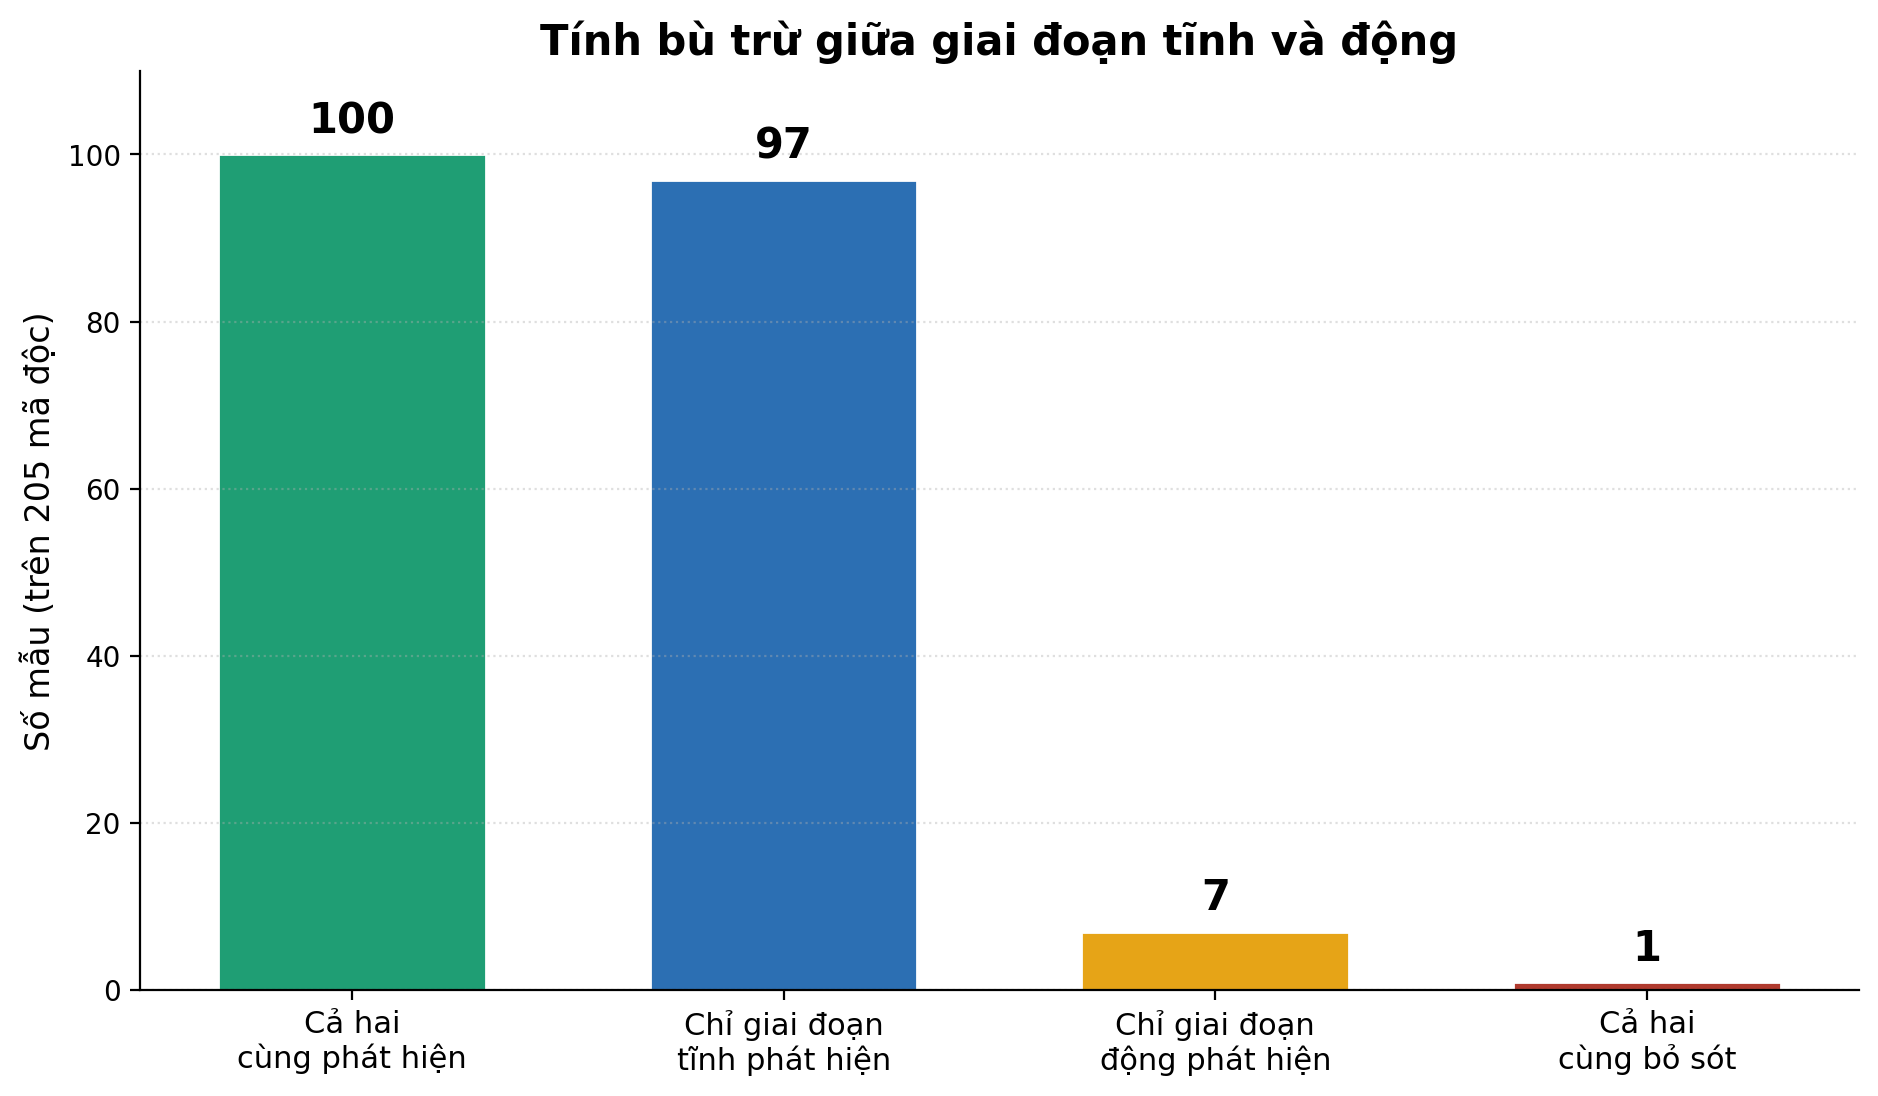
\includegraphics[width=1.0\textwidth]{Hinhve/Pic44Complementarity.png}
\caption{Tính bù trừ giữa giai đoạn tĩnh và động trên 205 mẫu mã độc.}
\label{fig:complementarity}
\end{figure}

Kết quả thực nghiệm cho thấy mô hình tĩnh Top-384 đạt F1 bằng 0{,}9615
trên EMBER 2024, giai đoạn động thu được bằng chứng hành vi cụ thể ở
72\% số mẫu, và khi hợp nhất hai giai đoạn hệ thống nhận diện đúng
204/205 mẫu mã độc --- minh chứng cho vai trò bù trừ của thiết kế
tĩnh--động. Những hạn chế còn lại và hướng phát triển được trình bày
ở phần Kết luận.

\end{document}
